\chapter{Conclusion and Outlook}

The software setup was created to investigate the energy behavior of the zone. Everything is build in the Rhino environment. This allows changes the geometry and observation of the resulting effects.
With little manual effort it is possible to investigate many orientations of the facade.\\
The completed simulations created a reliable setup. The chosen strategy to minimize the consumption hours by hours doesn't take into account the thermal inertia of the building, this aspect can reduce the precision of the obtained results.
Our results highlight that the optimal panels orientation will be a tradeoff between the three solutions we obtained. Inside this tradeoff solution a fourth parameter will play a fundamental role: the electricity production of the photovoltaics cells. It was not possible to integrate the calculation of this parameter in our setup because it is not yet implemented in DIVA for Grasshopper.\\
Figure~\ref{lady} has been obtained with ladybug (Rhinoceros3D additional tool) and suggest a promising way to calculate the solar irradiation.

\begin{figure}[h]
 \centering
 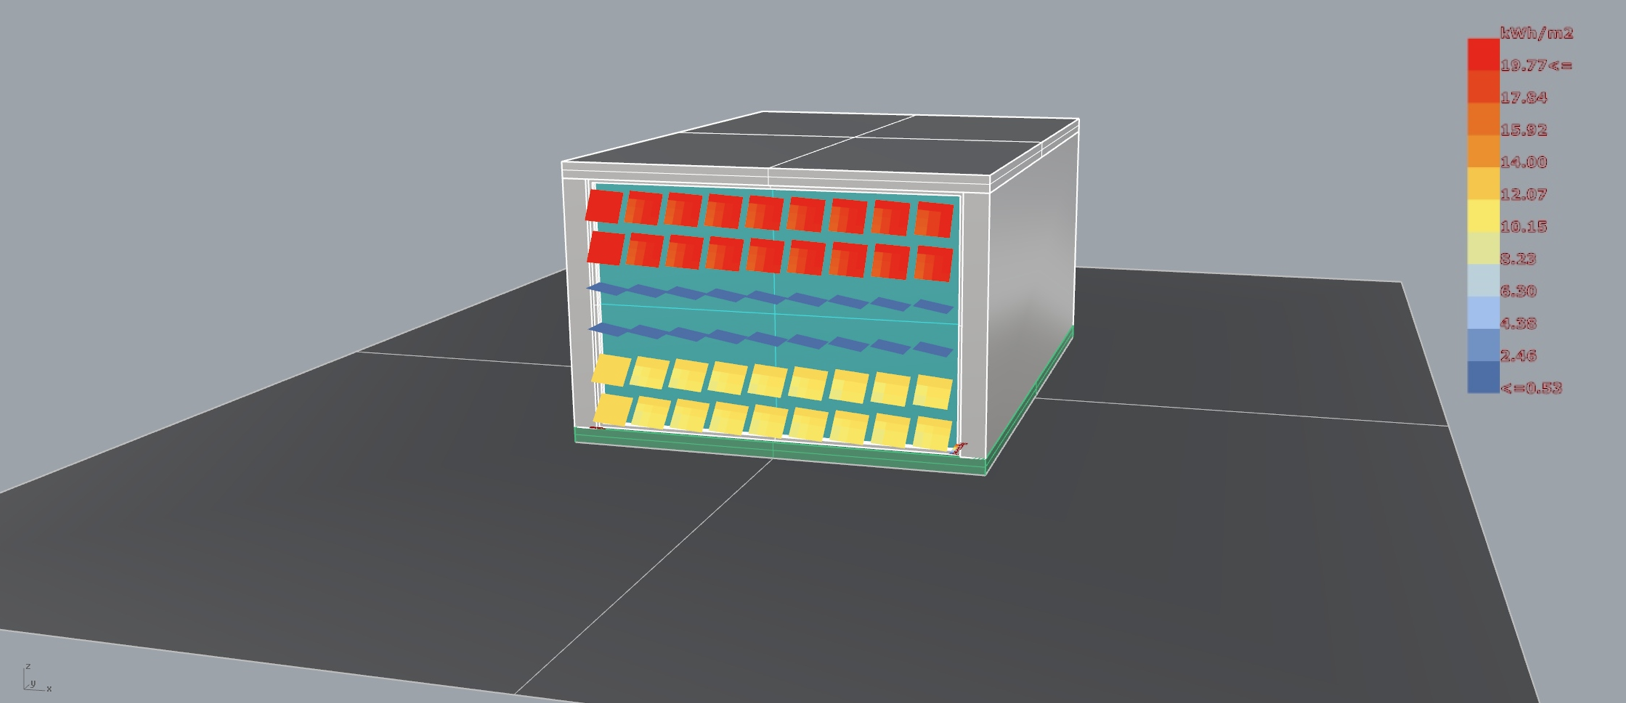
\includegraphics[width=150mm]{graphic/Ladybug_legend.png}
 \caption{Solar irradiation}
 \label{lady}
\end{figure}